\section{Quality Assurance}
% Organize this section according to major topics
% give each topic a section heading in boldface.
% try to cover the major common points :
%
% problem design
% methods of measurement
% supporting models
% supporting data
% simulations run
% results

% Just write the section headings for each part and indicate what goes in that
% section with words :
%
% heading
% figures (with captions)
% schematics (with captions and footnotes)
% equations
% tables

% What does it mean?
% What did I actually test?
% What were the results?
% Did the work yield a new method?
% Did the work yield new knowledge?
% What measurements did I make?
% How were these measurements characterized?
% What methods were used?
% What were the results?
% How were the measurements made and characterized?

Simulation science - like experimental science - has since the beginning had the 
problem of identifying trustworthy results from the nonsensical and the noise.
This is epitomized in the Charles Babbage quote, ``On two occasions I have been asked, 
`Pray, Mr. Babbage, if you put into the machine wrong figures, will the right 
answers come out?' ... I am not able rightly to apprehend the kind of confusion 
of ideas that could provoke such a question.'' \cite{babbage_passages_2011}. 
The \emph{garbage in, garbage out} phenomenon is not the only scenario which a
simulator must guard against; ensuring correctness is equally important.

Multiple strategies collectively known as \emph{\gls{QA}} have 
been invented over the years to mitigate the structural and algorithmic errors
on the part of simulators themselves. These include \emph{\gls{VV}}
\cite{boehm_software_1989}, \emph{\gls{UQ}} 
\cite{sacks_design_1989}, testing, and others. \gls{VV} and \gls{UQ} come from 
a distinctly computational science background while testing \emph{et al.} come from 
a software development bent. 

Nuclear engineering code quality is often governed by \gls{NQA1}, an 
\gls{ASME} specification 
whose latest revision appeared in 2009 \cite{asme_nqa-1a-2009_2009}. This is primarily 
used for designing reactors. However, it is general enough to apply to 
\Cyclus. \Cyclus has adopted an \emph{agile} development process 
\cite{larman_agile_2004}, 
interpreting \gls{NQA1} in a manner similar to the process adopted by the 
\gls{DOE} within \gls{NEAMS} \cite{neams_nuclear_2013} or the 
PyNE toolkit \cite{biondo_quality_2014}. 

\Cyclus acknowledges that quality assurance is an on-going process throughout the 
entire life of the code. As a simulator where most modeling decisions are made 
by third party archetype developers or users, the most important feature of 
\gls{QA} is verification. Validation may be impossible and \gls{UQ} is beyond 
he scope.

Verification may be defined as the question, ``Is \Cyclus being built correctly?'' 
To answer this question we turn to the software development of notions of testing,
documentation, version control, style guidelines, and continuous integration. 
This suite of process controls supplies mechanism for reliable and reproducible 
software. The impetus to implement these correctly is even stronger in a scientific 
context because of the emphasis on reproducibility and provenance. These are 
discussed below individually.

Validation on the other hand may be defined as the question, 
``Is \Cyclus the correct tool?''
Since \Cyclus is alone in its class as an agent-based fuel cycle simulator, longitudinal 
validation is not possible. Still code-to-code comparisons with fuel cycle
simulators with other modeling paradigms are underway, if nascent. However, such 
exercises are more likely to bring into relief the differences between the modeling
paradigms than be useful for QA and validation. 

Lastly, uncertainty quantification is a process that is used on specific simulation
instantiations to statistically determine its quality. Since the \Cyclus 
kernel requires an input file written by the user, \gls{UQ} is a process that applies 
more to those running \Cyclus than to those running it.  Furthermore, any 
\gls{UQ}
results that are generated are applicable only to the scenario that is under 
analysis. Thus for \Cyclus \gls{UQ} is well beyond the scope of core development.

Sections \ref{sec:qa-testing}-\ref{sec:qa-ci} discuss in greater detail the software 
development components that comprise the \Cyclus verification strategy.
Each of these on its own is a valuable addition to \gls{QA} but is cannot be the 
entire answer to the requirements imposed by \gls{NQA1}. Taken together and strictly 
adhered to they present a fortress through which undesirable code may siege, 
but never take.

\subsection{Testing}
\label{sec:qa-testing}

Automated software \emph{testing} is the first line of defense against
errors in implementation. It also acts as an early warning sign that the
simulator does or does not work as intended on a new system.
Testing serves a critical role in \gls{QA} because it directly compares the 
results of running software versus the expected behavior of the software.
In \Cyclus, three categories of tests are defined: unit tests, integration 
tests, and regression tests. 

It is important to note that before a proposed
code changes is allowed into main stream \Cyclus, all of the tests must pass
and the change must be covered by a test, either new or existing. This is 
matter of policy for the developers. Additionally, test code is equally likely 
as the code it is testing to contain errors. To prevent an infinite recursion 
of testing-the-tests, it is assumed that diligence and one level of testing 
is sufficient to meet the aims of the quality assurance.

\subsubsection{Unit Tests}

Unit tests are those which compare the results of the smallest code \emph{unit}, 
typically a single function or a class. What constitutes the smallest code
unit depends on the context of the specific unit in question. While this is 
an ambiguous definition, combined with a philosophy of keeping units as small
as possible it is often clear in practice what needs to be tested.

Cyclus uses the Google Test framework \cite{inc_googletest_2008} as a harness for running unit 
tests. Sufficient unit tests are required for any proposed change to the \Cyclus
code base. Currently \Cyclus implements over 450 unit tests and \Cycamore has 
85.  These cover approximately 65\% of their respective code bases. This number 
is expected to grow over time. 

\subsubsection{Integration Tests} 

Integration tests are any tests that combine multiple elements of the 
\Cyclus interface and test that they work correctly with each other.  By analogy, 
simply because the gears (units) are made correctly does not imply that the 
clock (integration) will run smoothly, run at all, or give the correct time.
In \Cyclus and \Cycamore, integration tests are performed by running sample
simulations and verifying that results are what would be expected ahead of 
time. Pre-canned input files have thus been constructed. Their results 
are inspected and compared via nose \cite{pellerin_nose_2007}, a Python test framework.
Python will run \Cyclus as a subprocess for each integration test. In this
way \Cyclus code units are tested in the full context that they will
executed. This category of testing is especially useful for ensuring that 
major \Cyclus components are functioning as expected.

\subsubsection{Regression Tests}

Regression tests are tests which ensure that significant changes do not 
occur over the course of \Cyclus development. Such a change is called a 
\emph{regression} because the new version is almost always wrong.
Regression tests are implemented similarly to integration tests.
Nose is used to execute fully fledged \Cyclus simulations whose results
are then compared. In this category however the comparison is done against 
the output of the same input file when run with a previous version of \Cyclus, 
typically the last released version.
In some sense, regression tests are `dumb' in that they do 
not care about the contents of a simulation being correct, only whether or not 
it changed. They thus pick up glaring time-sensitive mistakes that may 
not appear elsewhere though they do not purport to make claims about the
quality of the physics modeled. The \Cycamore project is the primary location of
regression tests. This is because the archetypes here are sophisticated enough
to make interesting input files. Only a handful ($<10$) time steps are needed 
for regression testing.

\subsection{Documentation}

All of the public interface (the \gls{API}) must be documented as part of \Cyclus
\gls{QA} policy. This certifies that the intention for a code unit is communicated 
in way that is separate from its implementation. This policy is important 
because implementations are often wrong, hence bugs. They are thus unreliable 
resources about themselves. Truly trustworthy communication about what 
software should be doing comes from the author explicitly stating the 
goals of an \gls{API} in prose form. Future development of the code is then able to 
compare the implementation versus the documentation to discern whether or not they 
are in agreement. Documentation is thus a secondary higher-level information 
stream.  In \Cyclus, this information is aggregated together into static 
websites with the Doxygen \cite{van_heesch_doxygen:_2008} and Sphinx 
\cite{brandl_sphinx_2014} 
tools. These websites are placed online at \url{http://fuelcycle.org}.

\subsection{Version Control}

Version control is the history-preserving mechanism by which the provenance of 
a code is recored. Cyclus uses a well-established tool called git 
\cite{software_freedom_conservancy_git_2014}
for this purpose. Git is currently the most popular utility in the recent wave
of \emph{distributed version control}. Briefly stated, this means that every 
user has a complete local copy of the \emph{repository} (the version control
term for the collection of all possible histories).
Though there and many praises and criticisms of git, one 
feature that the tool performs exceptionally well is the notion of code branches.
These are distinct pathways in the history that branch out of a mainline source
tree and then may be \emph{merged} back into the mainline. Multiple simultaneous
branches may exist at all point in time. Every change to the code is recorded
in the history, along with metadata such as the author, a timestamp, and an 
accompanying message. Thus 
it is possible for \Cyclus to accurately replay the entirety of who did what to the
code when.

Cyclus uses a strategy known as \emph{git flow} 
\cite{kalliamvakou_code-centric_2014} 
to manage topical branches where individuals develop code, the mainline development
branch (simply known as develop), and the stable branch (called master).
In addition to these rules and delineation, \Cyclus also imposes rules on 
when it is acceptable from a quality control standpoint to merge code from 
the personal topical branches into develop. All software at this stage 
must have sufficient and passing tests and comprehensive documentation. Without
these core pieces proposed changes are not allowed into \Cyclus. A schematic of 
the development stages between reporting a bug and merging the fix is shown in 
Figure \ref{fig:gitprocess}. 

\begin{figure}[htbp]
\begin{center}
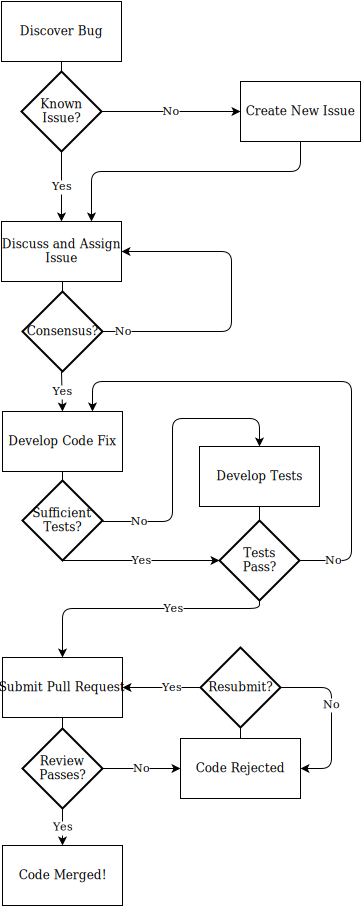
\includegraphics[height=0.6\textheight]{./images/gitprocess}
\end{center}
\caption{A version-control enabled process for finding, reporting, fixing a bug 
can take place within an issue tracker alongside multiple stages of code 
testing and review. In the \Cyclus case, the final review stage includes unit 
and integration testing as well as manual code inspection.}
\label{fig:gitprocess}
\end{figure}

The act of proposing a change is known as a \emph{pull request}. The main \Cyclus is 
hosted remotely on the GitHub website \cite{dabbish_social_2012}. The online
mechanism for pull requests allows for code review by a member of the \Cyclus 
core team other than the author prior to any change being included. Non-members
of the \Cyclus development team are allowed and encouraged to submit and review 
pull requests. However, only members of the \Cyclus core team are allowed to 
merge in any changes and only after the \gls{QA} standards have been met.

\subsection{Style Guide}

In any multi-person software project, there is a tension between how individuals
wish to write code. Every person tends to have their own custom style. To remedy this
coding style guides are the software analogy to the natural language ones, 
such as the Chicago Manual of Style. Cyclus strictly enforces the use of the 
Google C++ Style Guide \cite{weinberger_google_2008} for all software contributions.
This means that all developers of \Cyclus nominally write \Cyclus code in the same 
way.  This homogenization may be a hurdle to new developers but ultimately 
makes the it much more legible. Adoption of a single style guide also settles
timeless arguments over what style is `the best.' Having only one means that 
there is a common enemy for all developers to dislike equally.

\subsection{Continuous Integration}
\label{sec:qa-ci}

Continuous integration (CI) the idea that software should be tested and validated 
as it is being developed, rather than as a final stage in a longer development 
cycle.  Under CI every pull request is tested independently immediately after 
it is proposed. Such tests should be run on all officially supported platforms. 
Cyclus uses a CI platform called Polyphemus \cite{scopatz_polyphemus_2014}. 

Polyphemus serves as an intermediary between GitHub pull requests on the frontend 
and temporary \Cyclus servers on the backend. These servers are hosted by 
the Build \& Test Laboratory (BaTLab) \cite{uw_batlab_team_batlab_2014} at the University of 
Wisconsin-Madison. Whenever a pull request is created, Polyphemus performs 
the following actions:

\begin{enumerate}
    \item Copies \Cyclus with the pull requested code to BaTLab,
    \item Initializes Linux and Mac OSX servers,
    \item Builds \Cyclus on all platforms,
    \item Runs the complete \Cyclus test suite, 
    \item Reports back whether the above steps succeeded or not.
\end{enumerate}

Since these steps are performed for all incoming code, it is easy for the 
\Cyclus core team to determine whether or not an individual pull request 
actually works. This helps identify build and test problems prior to 
broken code being allowed into the develop branch.

CI has become a necessary but not sufficient addition to the \Cyclus \gls{QA}
system. Its merit is that it keeps bad code out. However, \Cyclus will always
require human eyes and human hands to let good code in.


